% !TEX root = ../report.tex
\chapter{Konzept}
\begin{Spacing}{\mylinespace}

\section{Modularisierung}
Um eine parallele Entwicklung und spätere Erweiterbarkeit sicherzustellen entschieden wir uns für eine modulbasierte Entwicklung.
Unser Projekt lässt sich in 3 Kategorien gliedern. Das ParticleSystem \textbf{(ParticleSystem)}, die Kinect Ansteuerung \textbf{(SandstormKinect)} und einen Controller \textbf{(Sandstorm)} der Events entgegen nimmt und diese verarbeitet oder ggf. weiterleitet.
Das XNA-Framework unterstützt einen modulbasierten Ansatz indem es jeder DrawableGameCompontent ihren eigenen Kontext zuweist.
Dies bedeutet das jede DrawableGameCompontent ein eigenes kleines Projekt darstellt und unabhängig von den anderen Projekten betrieben werden kann.
\begin{figure}[h!]
	\centering
	\vspace*{20px}
	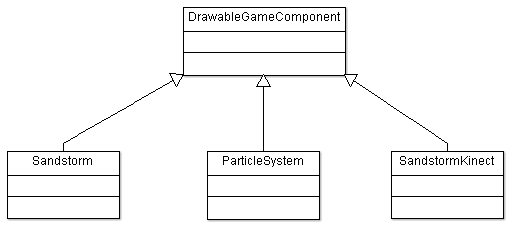
\includegraphics[width=320px]{graphics/DrawableGame.png}
	\caption{Kompontenten}
	\label{fig:singleColor}
\end{figure}

\section{Versionierung}
Um einen bestmöglichsten Konfort während der parallelen Entwicklung zu gewährleisten benötigt es eine Synchronisierung und Versionierung von Quellcode. Es gibt diverse Ansätze um dies sicherzustellen jedoch bietet Tools wie SVN, CVS, Perforce oder GIT sehr ähnliche Funktionlitäten. Wir entschieden uns aus Gewohnheit für ein GIT-Repository auf Github.com, dies lies sich innerhalb von Minuten einrichten und ist überall - sofern eine Internetverbindung besteht erreichbar. Jeglicher Quellcode des Projekts lässt sich somit unter folgender Adresse abrufen: \url{https://github.com/tsturm/sandstorm}. Zusätzlich wird auf dem Perforce-Server des Fachbereichs Informatik die aktuelle Version vorgehalten.

\end{Spacing}
\newpage
\clearpage
%% End Of Doc